\documentclass[9pt]{beamer}
%\usepackage{amsmath,amssymb,amsthm,tikz-cd}
\usetheme{Madrid}
\usecolortheme{default}
\DeclareMathOperator{\Hom}{Hom}
\DeclareMathOperator{\Det}{det}
\DeclareMathOperator{\supp}{supp}

\title[Differentiable manifolds and the Hairy Ball Theorem]
{Differentiable manifolds and the Hairy Ball Theorem}

\author[Jonathan Lau] % (optional)
{Jonathan Lau}

\AtBeginSection[]
{
	\begin{frame}
		\frametitle{Table of Contents}
		\tableofcontents[currentsection]
	\end{frame}
}

\begin{document}
	
\frame{\titlepage}

\begin{frame}
	\frametitle{Table of Contents}
	\tableofcontents
\end{frame}

\section{Manifolds}
	
\begin{frame}{Stokes' Theorem}
    Stokes' Theorem:\[\int_Md\omega = \int_{\partial M} \omega\]

    Special cases: \[\int_{\partial D} Pdx+Qdy = \int_D \left(\frac{\partial Q}{\partial x}-\frac{\partial P}{\partial y}\right) dA\]
    \[\int_{\partial V}  F\cdot dS = \int_V \text{div} F\]
\end{frame}

\begin{frame}
    \begin{block}{Upper Half Space}
        The upper half space is $\mathcal{H}^n=\{(x_1, \dots, x_n)\in \mathbb{R}^n\mid x_n >= 0\}$. Its boundary is $\partial \mathcal{H}^n = \{(x_1, \dots, x_n)\in \mathbb{R}^n\mid x_n = 0\}$.
    \end{block}
    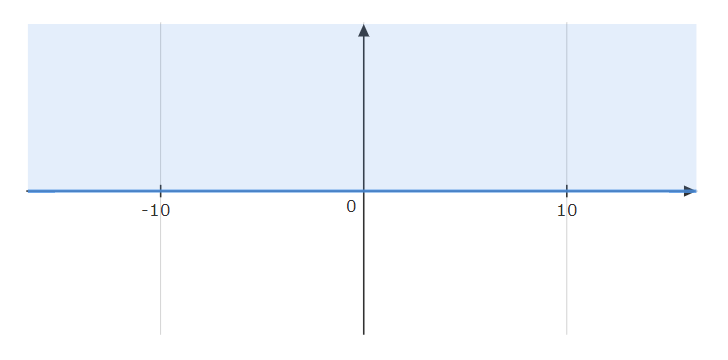
\includegraphics[scale=0.6]{upper_half.PNG}

\end{frame}
\begin{frame}
    \begin{block}{Charts}
        A chart on a topological space $M$ is a pair $(U, \phi)$ consisting of an open $U\subset M$ and a homeomorphism $\phi:U\rightarrow V\subset\mathbb{H}^n$.
    \end{block}

    We can express $\phi$ as $(x_1, \dots, x_n)$.

    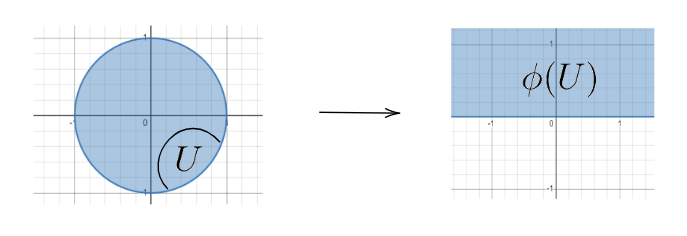
\includegraphics[scale=0.6]{chart.PNG}

    Example: sphere
    
\end{frame}

\begin{frame}
    \begin{block}{Manifolds with boundary}
        A $n$ dimensional manifold with boundary $M$ is a subset of $\mathbb{R}^\ell$ together with a collection of charts $\mathcal{A}$ that cover $M$ such that for all charts $(U, \phi)$, $(V, \psi)$, the maps $\psi\circ\phi^{-1}$ and $\phi\circ\psi^{-1}$ are smooth on $\phi(U\cap V)$ and $\psi(U\cap V)$ respectively.

        Such a collection is called an atlas.
    \end{block}
    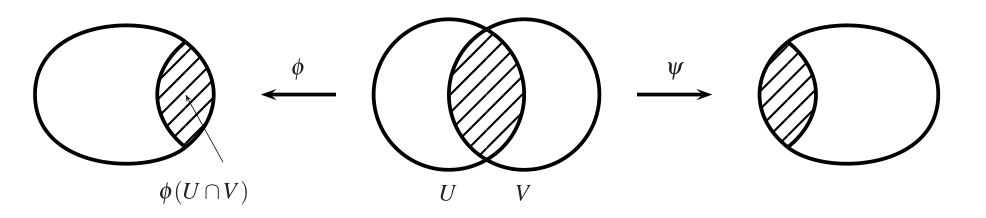
\includegraphics[scale=0.55]{compatible.PNG}

\end{frame}

\begin{frame}{}
    \begin{block}{Boundary}
        Let $M$ be a manifold with boundary. A point $p$ is a boundary point if for some chart $(U, \phi)$, $\phi(p)\in \partial \mathcal{H}^n$. The set of all boundary points is the boundary $\partial M$.
    \end{block}


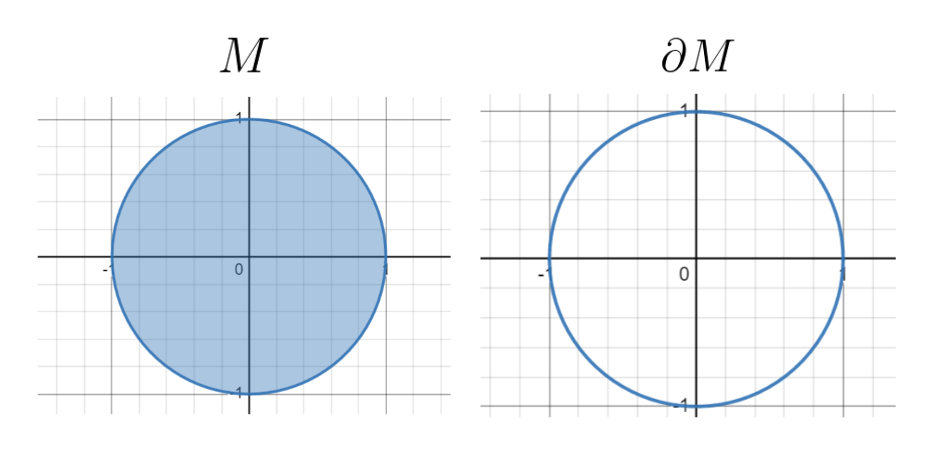
\includegraphics[scale=0.6]{boundaryPNG.PNG}

\end{frame}
\begin{frame}
    \begin{block}{Manifold}
        A manifold with boundary $M$ with empty boundary is called a manifold. 
    \end{block}

    \begin{block}{Proposition: Boundary is manifold}
        Let $M$ be a manifold with boundary. Then, $\partial M$ is a manifold.
    \end{block}
    proof: Let $\mathcal{A}$ be an atlas on $M$. For each $(U, x_1, \dots, x_n)\in \mathcal{A}$, we construct a chart on $(U\cap \partial M , x_1|_{\partial M}, \dots, x_{n-1}|_{\partial M})$ on $\partial M$.
\end{frame}

\begin{frame}
    \begin{block}{Tangent Space}
        Let $M$ be a manifold. Given a point $p\in M$ and a smooth curve $\gamma:(-1,1)\rightarrow M$ in $M$ such that $\gamma(0)=p$, its velocity vector is $\frac{d\gamma}{dt}\vert_{t=0}$. The set of all velocity vectors at $p$ is the tangent space at $p$, denoted $T_p M$.
    \end{block}
    Let $(U, \phi)$ with $\phi(p)=0$, and let $\gamma_i:t\mapsto \phi^{-1}\circ\iota_i(t)$. Then, $e_i=\frac{\partial \gamma_i}{\partial t}$ form a basis for $T_pM$. We call this the basis induced by $\phi$.
\begin{center}
    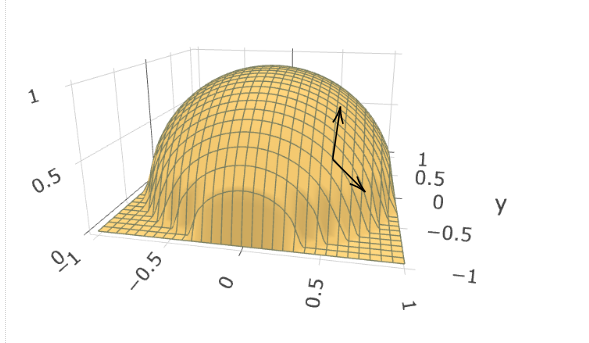
\includegraphics[scale=0.8]{tangent_vectors.png}
\end{center}
\end{frame}

\begin{frame}
    \begin{block}{Smooth Functions}
        Let $N,M$ be manifolds. A continuous function $F:N\rightarrow M$ is smooth if for all charts $(U, \phi)$ on $N$ and $(V, \psi)$ on $M$, $\psi\circ F\circ \phi^{-1}$ is smooth.
    \end{block}
    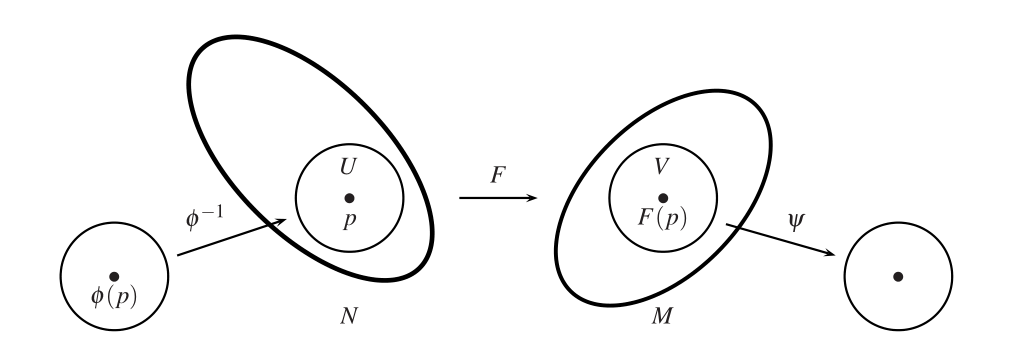
\includegraphics[scale=0.55]{smooth_function.PNG}
\end{frame}

\begin{frame}{}
    \begin{block}{Differential}
        Let $F: N \rightarrow M$ be a smooth function, $p\in N$, and $(U, x_1,\dots,x_n)$, $(V, y_1,\dots,y_m)$ are charts on $N$ and $M$. Let $v\in T_pM$. Then, there exists a curve $\gamma$ such that $\frac{d \gamma}{d t} = v$. We define the differential $F_*(v)=\frac{d F\circ\gamma}{d t}$.
    \end{block}    

    In the bases induced by $\phi, \psi$, the differential $F_*:T_pM \rightarrow T_{F(p)}N$ at $p$ is a linear transformation represented by the matrix $J(\psi\circ F\circ \phi^{-1})$, where $J(f)=\left(\frac{\partial f_i}{\partial x_j}\right)$ is the $m$ by $n$ Jacobian matrix.
    

    Example: $F:S^2 \rightarrow \mathbb{R}^3, (x,y,z)\mapsto (2x,y,z)$, $p=1/3(1,2,2)$, $\phi:(x,y,z)\mapsto (x,y)$, $\psi:(x,y,z)\mapsto (x,y)$.
\end{frame}

\begin{frame}
    \begin{block}{1-form}
        Let $(U, \phi)$ be a chart on $M$. A 1-form $\omega$ is a linear function from $T_p M$ to $\mathbb{R}$.
    \end{block}
    $\Hom(T_p M, \mathbb{R})\equiv \mathbb{R}^n$. Fixing a basis for $T_pM$, we define $(dx_i)_p(a_1, \dots, a_n) = a_i$.
    \begin{block}{$k$-form}
        Let $(U, \phi)$ be a chart on $M$. A $k$-form $\omega$ is an alternating multilinear function from $(T_p M)^k$ to $\mathbb{R}$.
    \end{block}

\end{frame}

\begin{frame}
    \begin{block}{Wedge Product}
        The wedge product of $k$ 1-forms $\omega_1, \dots, \omega_k$ is the k-form $\omega_1\wedge\dots\wedge\omega_k(v_1, \dots, v_k)=\Det(\omega_i(v_j))$.
    \end{block}
    On $T_p\mathbb{R}^5$, $dx_1\wedge dx_3((0,0,1), (2,2,2))=\Det\begin{pmatrix} 0 & 2 \\
        1 & 2
    \end{pmatrix}$. This is the same as projecting $(0,0,1), (2,2,2)$ onto the $x-z$ plane, then calculating it's area.
    
    \begin{block}{Theorem}
        $\{(dx_{i_1})_p\wedge\dots\wedge (dx_{i_k})_p|1\leq i_i<\dots<i_k\leq n\}$ is a basis for $\Lambda^k(T_pM)$, the set of alternating multilinear functions on $(T_pM)^k$.
    \end{block}
    So, $(dx_1)_p, \dots, (dx_n)_p$ is a basis for $\Hom(T_p M, \mathbb{R})$, and $(dx_1)_p\wedge\dots\wedge (dx_n)_p$ is a basis for $\Lambda^n(T_pM)$, i.e. every $\omega\in\Lambda^n(T_pM)$ is a multiple of $(dx_1)_p\wedge\dots\wedge (dx_n)_p$.
\end{frame}

\begin{frame}
    \begin{block}{Differential Forms}
        A differential $k$-form $\omega$ is a function $\omega: p\in M \mapsto \omega_p\in\Lambda^kT_pM$, and for all charts $(U, x_1, \dots, x_n)$, $\omega_p=\sum_I f_I(p)dx_I$ on $U$ for some smooth $f_i$'s.
    \end{block}

    Example: $dx_I$ is a differential $k$-form.

    \begin{block}{The $d$ operator}
        Let $f:M\rightarrow \mathbb{R}$ be a smooth function. We define a differential 1-form $df$ as $\sum_{i=1}^n \frac{\partial f}{\partial x_i}dx_i$.
        Given a differential form $\omega$ on $M$ and a chart $(U, \phi)$, $\omega=\sum_I f dx_I$ on $U$. Then, on $U$, $d\omega$ is defined as $\sum_I df\wedge dx_I$.
    \end{block}

\end{frame}

\section{Integration of Differential \texorpdfstring{$n$}{n}-Forms}
\begin{frame}
    \begin{block}{Orientation}
        An orientation on a manifold with boundary is a non-vanishing differential $n$-form.
    \end{block}

    \begin{block}{Oriented Atlas}
        An oriented atlas is an atlas $\mathcal{A}$ such that for all $(U, \phi),(V, \psi)\in \mathcal{A}$, $\Det(J(\psi\circ\phi ^{-1}))>0$.
    \end{block}

    \begin{block}{Theorem}
        \[\text{Orientations} \iff \text{Oriented atlas}\]
        \[ \omega \iff \omega_p(e_1,\dots,e_n)>0,\] where $e_1,\dots,e_n$ is the basis induced by $(U, \phi)$.
    \end{block}
\end{frame}

\begin{frame}
    \begin{block}{Integration on a $\mathbb{R}^n$}
        Let $\omega$ be a $n$-form on $(U, \phi)$, where $U\subset\mathbb{R}^n$. Then $\omega=f(x)dx_1\wedge\dots\wedge dx_n$ for some smooth $f$. The integral of $\omega$ over $U$ is $\int_U\omega=\int_U f$.
    \end{block}

    \begin{block}{Pullback}
        Let $\omega_p\in \Lambda^kT_pM$ and $F:N \rightarrow  M$. The pullback of $\omega_p$ by $F$ is $F^*(\omega_p)\in \Lambda^kT_pN$, defined as \[F^*(\omega_p)(v_1,\dots,v_k)=\omega_p(F_*(v_1),\dots, F_*(v_k)).\]
        The pullback of a differential form $\omega$ is defined as $(F^*\omega)_p=F^*(\omega_p)$.
    \end{block}

    \begin{block}{Integration on a chart}
        Let $\omega$ be a $n$-form on $(U, \phi)$. The integral of $\omega$ over $U$ is $\int_U\omega=\int_{\phi(U)}(\phi^{-1})^*\omega$. 
    \end{block}
\end{frame}

\begin{frame}
    \begin{block}{Partition of Unity}
        A partition of Unity on a manifold $M$ is a collection of nonnegative smooth functions $\{\rho_\alpha:M \rightarrow \mathbb{R}\}_{\alpha\in A}$ such that \begin{enumerate}[i]
            \item the collection of supports, $\{\supp\rho_\alpha\}_{\alpha\in A}$, is locally finite,
            \item $\sum_{\alpha\in A} \rho_\alpha = 1.$
        \end{enumerate}
    \end{block}

    \begin{block}{Integration on a Manifold}
        Let $\omega$ be a $n$-form on $M$. The integral of $\omega$ over $M$, denoted by $\int_M \omega$, is defined to be $\sum_{\alpha\in A}\int_{U_\alpha}\rho_\alpha\omega$.
    \end{block}
\end{frame}

\begin{frame}
    \begin{block}{Stokes' theorem on $\mathcal{H}^n$}
        stuff ...
    \end{block}
\end{frame}

\begin{frame}
    \begin{block}{Stokes' theorem on Manifolds}
        stuff ...
    \end{block}
\end{frame}

\end{document}